\documentclass{article}
\usepackage{tikz}
\usepackage{graphicx}
\usepackage{tkz-euclide}
\usepackage{gensymb}
\usepackage{array}
\usepackage[lofdepth,lotdepth]{subfig}
\usetikzlibrary{angles,through,calc,intersections}

\begin{document}
\begin{enumerate}

\item During the lockdown period, many families got bored of watching TV all the time. Out of these families, one family of 6 members decided to play a card game. 17 cards numbered 1, 2, 3, 4, ..., 17 are put in a box and mixed thoroughly. One card is drawn by one member at random and other family members bet for the chances of drawing the number either prime, odd or even etc.     
	
	\begin{figure}[!h]
	\centering
	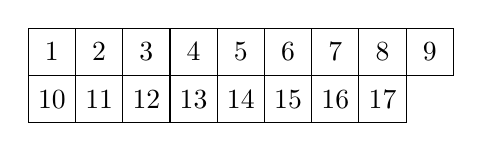
\begin{tikzpicture}
  \def\gridsize{9}
  \def\boxsize{0.6}
  \foreach \i in {1,...,\gridsize} {
  \pgfmathtruncatemacro\boxnumber{\i}
  \draw (\i*\boxsize, 0) rectangle ++(\boxsize, -\boxsize);
  \node at (\i*\boxsize+0.5*\boxsize, -0.5*\boxsize) {\boxnumber};
  }
  \def\gridsize{8}
  \foreach \i in {1,...,\gridsize} {
  \pgfmathtruncatemacro\boxnumber{\i+9}
  \draw (\i*\boxsize, -\boxsize) rectangle ++(\boxsize, -\boxsize);
  \node at (\i*\boxsize+0.5*\boxsize, -1.5*\boxsize) {\boxnumber};
  }
\end{tikzpicture}

	\caption{Caption}
	\label{fig:0}
        \end{figure}
	
	\begin{figure}[h!]
	\centering
	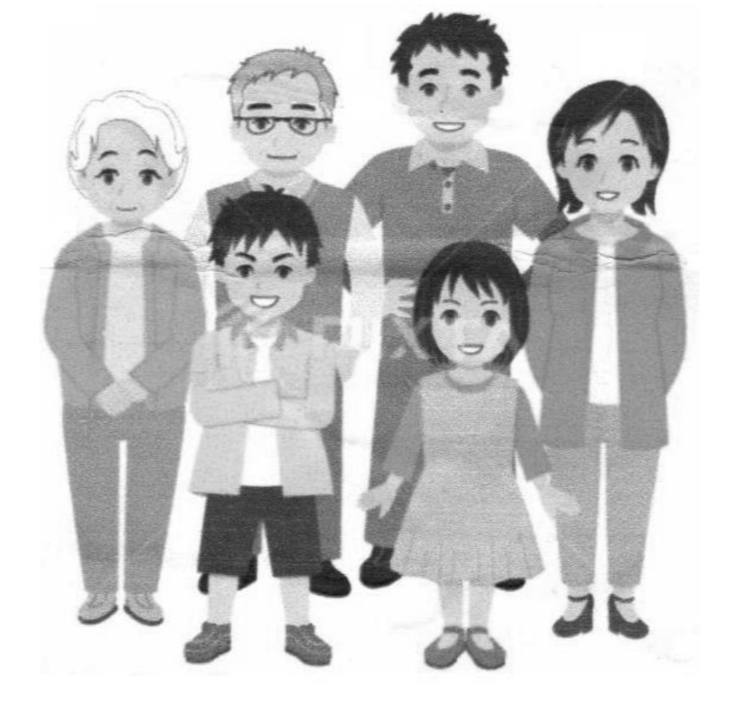
\includegraphics[width=\columnwidth]{figs/1.jpg}
	\caption{A family representation}
	\label{fig:1}
	\end{figure} 
Based on the above, answer the following questions : 		
\begin{enumerate}
\item The first member of the family draws a card at random and another member bets that it is an even prime number. What is the probability of his winning the bet ? 
	\begin{enumerate}
	\item $\frac{2}{17}$
	\item $\frac{3}{17}$
	\item $\frac{1}{17}$ 
	\item $\frac{4}{17}$ 
	\end{enumerate}
\item The second member of the family draws a card at random and some other member bets that it is an even number. What is the probability of his winning the bet ? 
	\begin{enumerate}
	\item $\frac{7}{17}$
	\item $\frac{8}{17}$
	\item $\frac{9}{17}$ 
	\item $\frac{10}{17}$ 
	\end{enumerate}
\item What is the probability that the number on the card drawn at random is divisible by 5 ? 
	\begin{enumerate}
	\item $\frac{5}{17}$
	\item $\frac{4}{17}$
	\item $\frac{3}{17}$ 
	\item $\frac{2}{17}$ 
	\end{enumerate}
\item What is the probability that the number on the card drawn at random is a multiple of 3 ? 
	\begin{enumerate}
	\item $\frac{5}{17}$
	\item $\frac{6}{17}$
	\item $\frac{7}{17}$ 
	\item $\frac{8}{17}$ 
	\end{enumerate}
\item What is the probability that the number on the card is a factor of 9 ?
	\begin{enumerate}
	\item $\frac{9}{17}$
	\item $\frac{3}{17}$
	\item $\frac{8}{17}$ 
	\item $\frac{1}{17}$ 
	\end{enumerate}
\end{enumerate}
		
\item Find the distance between the points $ \vec{A} (-\frac{7}{3},5) $ and $ \vec{B} (\frac{2}{3},5) $. 

\item Check whether $13$ cm, $12$ cm, $5$ cm can be the sides of a right triangle.
		
\item If $ \vec{PL} $ and $ \vec{PM} $ are two tangents to a circle with centre O from an external point $\vec{P}$ and $PL = 4 cm$, find the length of OP, where radius of the circle is $3$ cm.
			
\item Find the distance between two parallel tangents of a circle of radius $2·5$ cm. 

\item Find the coordinates of the point which divides the line segment joining the points $\vec{A}(7, 1)$ and $\vec{B}( 3, 4)$ in the ratio $2 : 3$. 

\item Show that the points $\vec{A}(1,7), \vec{B}(4,2), \vec{C}(1,1), \vec{D}(4,4)$ are the vertices of a square $ABCD$. 

\item A quadrilateral $ABCD$ is drawn to circumscribe a circle Fig.\ref{fig:2}. Prove that $ AB + CD = AD + BC. $
	\begin{figure}[h]
	\centering
	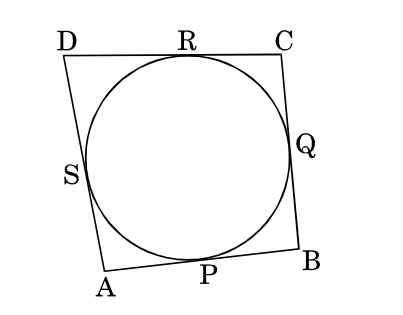
\includegraphics[width=\columnwidth]{figs/2.jpg}
	\caption{A circle inscribed in a quadrilateral}
	\label{fig:2}
	\end{figure}

\item Draw a pair of tangents to a circle of radius $4$ cm which are inclined to each other at an angle of $40\degree$. 

\item To divide a line segment $QP$ internally in the ratio of $2 : 3$, we draw a ray $\vec{QY}$ such that $\angle PQY$ is acute. What will be the minimum number of points to be located at equal distances on the ray $\vec{QY}$ ? 

\item Answer any \textbf{\textit{four}} of the following questions : 		
\begin{enumerate}
\item The point which divides the line segment joining the points $(7, 6)$ and $(3, 4)$ in the ratio $1 : 2$ lies in
	\begin{enumerate}
	\item I quadrant 
	\item II quadrant 
	\item III quadrant  
	\item IV quadrant
	\end{enumerate}
\item  If the points $\vec{A}(1, 2), \vec{O}(0, 0)$ and $\vec{C}(a, 6)$ are collinear, then the value of a is 
	\begin{enumerate}
	\item 6
	\item $\frac{3}{2}$
	\item 3
	\item 12
	\end{enumerate}
\item  The distance between the points $\vec{A}(0, 6)$ and $\vec{B}(0, 2)$ is 
	\begin{enumerate}
	\item 6 units
	\item 8 units
	\item 4 units
	\item 2 units
	\end{enumerate}
\item  If $(\frac{a}{3},4)$ is the mid-point of the line segment joining the points $(-6, 5)$ and $(-2, 3)$, then the value of ${\lq a\rq}$ is
	\begin{enumerate}
	\item -4
	\item 4
	\item -12
	\item 12
	\end{enumerate}
\item  What kind of triangle is formed with vertices $\vec{A}(0, 2)$, $\vec{B}(3, 0)$ and $\vec{C}(3, 0)$ ? 
	\begin{enumerate}
	\item A right triangle 
	\item An equilateral triangle
	\item An isosceles triangle 
	\item A scalene triangle 
	\end{enumerate}
\end{enumerate}
		
\item  If the distance between the points $(k, 2)$ and $(3,-6)$ is $10$ units, find the positive value of $k$. 
			
\item  Find the length of the segment joining $\vec{A}(-6, 7)$, and $\vec{B}(-1, -5)$,. Also, find the mid-point of $AB$. 
	
\item  A point $\vec{T}$ is $13 cm$ away from the centre of a circle. The length of the tangent drawn from $\vec{T}$ to the circle is $12$ cm. Find the radius of the circle. 
	
\item  Two tangents $ \vec{TP} $ and $ \vec{TQ} $ are drawn to a circle with centre O from an external point T. Prove that $\angle PTQ= 2 \angle OPQ$. 

\item  A man goes $5$ metres due West and then $12$ meters due North. How far is he from the starting point?

\item Students of a school are standing in rows and columns in their school playground to celebrate their annual sports day. $\vec{A}$, $\vec{B}$, $\vec{C}$ and $\vec{D}$ are the positions of four students as shown in the Fig.\ref{fig:3}

	\begin{figure}[!h]
	\centering
	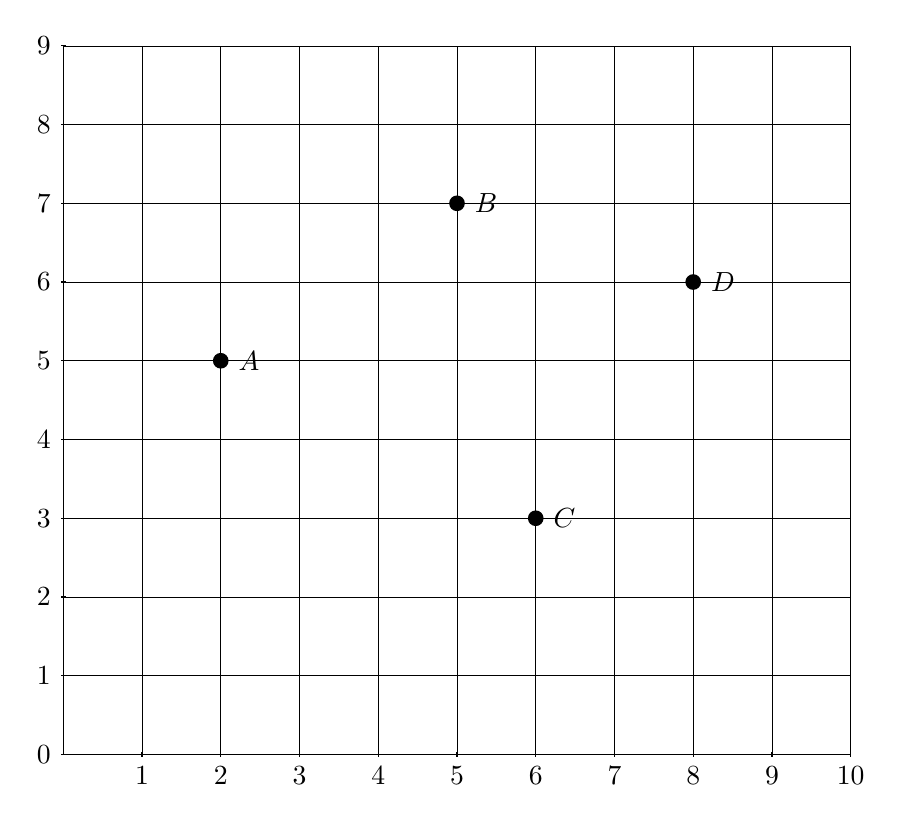
\begin{tikzpicture}
    \draw[step=1cm,very thin]  grid (10,9);
    \foreach \x in {1,2,3,4,5,6,7,8,9,10}
    \draw (\x cm,1pt) -- (\x cm,-1pt) node[anchor=north] {$\x$};
    \foreach \y in {0,1,2,3,4,5,6,7,8,9}
    \draw (1pt,\y cm) -- (-1pt,\y cm) node[anchor=east] {$\y$};
    \node[shape=circle,fill=black, label=right:$A$,scale=0.6] (1) at (2,5){} ;
    \node[shape=circle,fill=black, label=right:$B$,scale=0.6] (1) at (5,7){} ;
    \node[shape=circle,fill=black, label=right:$C$,scale=0.6] (1) at (6,3){} ;
    \node[shape=circle,fill=black, label=right:$D$,scale=0.6] (1) at (8,6){} ;
 \end{tikzpicture}

	\caption{Caption}
	\label{fig:3}
        \end{figure}	
	
Based on the above, answer the following questions : 	
\begin{enumerate}
\item  The figure formed by the four points $\vec{A}$, $\vec{B}$, $\vec{C}$ and $\vec{D}$ is a 
	\begin{enumerate}
	\item  square 
	\item  parallelogram
	\item  rhombus 
	\item  quadrilateral 
	\end{enumerate}
\item If the sports teacher is sitting at the origin, then which of the four students is closest to him? 
	\begin{enumerate}
	\item  A
	\item  B
	\item  C
	\item  D
	\end{enumerate}
\item The distance between $\vec{A}$ and $\vec{C}$ is
	\begin{enumerate}
	\item $\sqrt{37}$ units
	\item $\sqrt{35}$ units
	\item 6 units
	\item 5 units
	\end{enumerate}
\item The coordinates of the mid-point of line segment $AC$ are
	\begin{enumerate}
	\item $(\frac{5}{2},11)$
	\item $(\frac{5}{2},\frac{11}{2})$
	\item $(5,\frac{11}{2})$
	\item $(5,11)$
	\end{enumerate}
\item If a point $\vec{P}$ divides the line segment $AD$ in the ratio 1 : 2, then coordinates of $\vec{P}$ are
	\begin{enumerate}
	\item $(\frac{8}{3},\frac{8}{3})$
	\item $(\frac{10}{3},\frac{13}{3})$
	\item $(\frac{13}{3},\frac{10}{3})$
	\item $(\frac{16}{3},\frac{11}{3})$
	\end{enumerate}
\end{enumerate}
		
\item Check whether the points $\vec{P}(5, 2)$, $\vec{Q}(6, 4)$, $\vec{R}(7, 2)$ are the vertices of an isosceles triangle $PQR$.

\item Find the ratio in which $\vec{P}(4, 5)$ divides the join of $\vec{A}(2, 3)$ and $\vec{B}(7, 8)$. 
	
\item $\vec{PQ}$ is a tangent to a circle with centre O at the point P on the circle. If $\triangle OPQ$ is an isosceles triangle, then find $\angle OQB$. 

\item Two concentric circles have radii $10$ cm and $6$ cm. Find the length of the chord of the larger circle which touches the smaller circle. 

\item If tangents $\vec{PA}$ and $\vec{PB}$ from an external point $\vec{P}$ to a circle with centre O are inclined to each other at an angle of $70\degree$, then find $\angle POA$. 

\item ABC is right triangle, right-angled at B, with $BC = 6$ cm and $AB = 8$ cm. A circle with centre O and radius $r$ cm has been inscribed in $\triangle ABC$ as shown in the Fig.\ref{fig:4}. Find the value of $r$. 
	\begin{figure}[h]
	\centering
	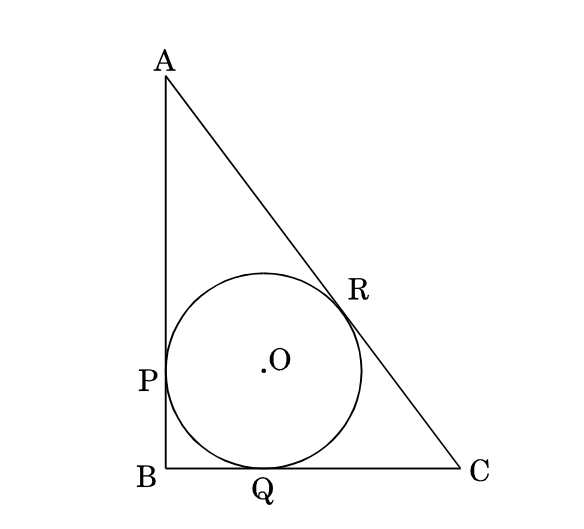
\includegraphics[width=\columnwidth]{figs/3.jpg}
	\caption{A circle inscribed in a triangle}
	\label{fig:4}
	\end{figure}
	
\item If the graph of a pair of lines $x - 2y + 3 = 0$ and $2x - 4y = 5$ be drawn, then what type of lines are drawn ? 
  
\item The coordinates of the three consecutive vertices of a parallelogram $ABCD$ are $\vec{A}(1, 3)$, $\vec{B}(-1, 2)$ and $\vec{C}(2, 5)$. Find the coordinates of the fourth vertex $\vec{D}$. 

\item If $\vec{P}(2, 2)$, $\vec{Q}(-4, -4)$ and $\vec{R}(5, -8)$ are the vertices of a $\triangle PQR$, then find the length of the median through $\vec{R}$.

\item Find the ratio in which the y-axis divides the line segment joining the points $\vec{A}(5, -6)$ and $\vec{B}(-1, -4)$. Also, find the coordinates of the point of intersection.

\item Find the ratio in which the line segment joining the points $\vec{A}(1, -5)$ and $\vec{B}(-4, 5)$ is divided by the x-axis. Also, find the coordinates of the point of division.
   
\item The points $\vec{A}(0, 3)$, $\vec{B}(-2, a)$ and $\vec{C}(-1, 4)$ are the vertices of a right triangle, right-angled at $\vec{A}$. Find the value of $a$. 
		
\item In a right triangle $ABC$, right-angled at $B$, $BC = 6 cm$ and $AB = 8$ cm. A circle is inscribed in the $\triangle ABC$. Find the radius of the incircle. 
			
\item Two circles touch externally at $\vec{P}$ and $ \vec{AB} $ is a common tangent, touching one circle at $\vec{A}$ and the other at $\vec{B}$. Find the measure of $\angle APB$.

\item From an external point $\vec{P}$, tangents $\vec{PQ}$ and $\vec{PR}$ are drawn to a circle with centre O, touching the circle at $\vec{Q}$ and $\vec{R}$. If $\angle QOR$ = $140\degree$, find the measure of $\angle QPR$. 

\item A circle touches all the sides of a quadrilateral $ABCD$. Prove that $AB + CD = DA + BC$.

\item Write the steps of construction of a circle of diameter $6$ cm and drawing of a pair of tangents to the circle from a point $5$ cm away from the centre. 
		
\end{enumerate}	
\end{document}
